\chapter{Special functions in genr}
\label{chap-genr}

\section{Introduction}
\label{genr-intro}

The \verb+genr+ command provides a flexible means of defining new
variables.  It is documented in the \GCR.  This chapter offers a more
expansive discussion of some of the special functions available via
\verb+genr+ and some of the finer points of the command.
    
\section{Long-run variance}
\label{sec:lrvar}

As is well known, the variance of the average of $T$ random variables
$x_1, x_2, \ldots, x_T$ with equal variance $\sigma^2$ equals
$\sigma^2/T$ if the data are uncorrelated. In this case, the sample
variance of $x_t$ over the sample size provides a consistent estimator.

If, however, there is serial correlation among the $x_t$s, the
variance of $\bar{X} = T^{-1} \sum_{t=1}^T x_t$ must be estimated
differently. One of the most widely used statistics for this purpose
is a nonparametric kernel estimator with the Bartlett kernel defined
as
\begin{equation}
  \label{eq:scalar-lrvar}
  \hat{\omega}^2(k) = T^{-1} \sum_{t=k}^{T-k} \left[ \sum_{i=-k}^k w_i (x_t -
  \bar{X}) (x_{t-i} - \bar{X}) \right] ,
\end{equation}
where the integer $k$ is known as the window size and the $w_i$ terms
are the so-called \emph{Bartlett weights}, defined as $w_i = 1 -
\frac{|i|}{k + 1}$. It can be shown that, for $k$ large enough,
$\hat{\omega}^2(k)/T$ yields a consistent estimator of the variance of
$\bar{X}$.

\app{Gretl} implements this estimator by means of the function
\texttt{lrvar()}, which takes two arguments: the series whose long-run
variance must be estimated and the scalar $k$. If $k$ is negative, the
popular choice $T^{1/3}$ is used.

\section{Time-series filters}
\label{sec:filters}

One sort of specialized function in \verb+genr+ is time-series
filtering. In addition to the usual application of lags and
differences, \app{gretl} provides fractional differencing and two
filters commonly used in macroeconomics for trend-cycle decomposition:
the Hodrick--Prescott filter \citep{hodrick97} and the Baxter--King
bandpass filter \citep{baxter-king99}.

\subsection{Fractional differencing}
\label{sec:fracdiff}

The concept of differencing a time series $d$ times is pretty obvious
when $d$ is an integer; it may seem odd when $d$ is
fractional. However, this idea has a well-defined
mathematical content: consider the function
\[
  f(z) = (1 - z)^{-d},
\]
where $z$ and $d$ are real numbers. By taking a Taylor series
expansion around $z=0$, we see that
\[
  f(z) = 1 + dz + \frac{d (d+1)}{2} z^2 + \cdots 
\]
or, more compactly,
\[
  f(z) = 1 + \sum_{i=1}^{\infty} \psi_i z^i
\]
with
\[
  \psi_k = \frac{\prod_{i=1}^{k} (d+i-1) }{k!} = \psi_{k-1} \frac{d+k-1}{k}
\]

The same expansion can be used with the lag operator, so that if we defined
\[
  Y_t = (1-L)^{0.5} X_t
\]
this could be considered shorthand for
\[
Y_t = X_t - 0.5 X_{t-1} - 0.125 X_{t-2} - 0.0625 X_{t-3} - \cdots 
\]
    
In \app{gretl} this transformation can be accomplished by the syntax 
\begin{code}
genr Y = fracdiff(X,0.5)
\end{code}

\subsection{The Hodrick--Prescott filter}
\label{sec:hodrick-prescott}

This filter is accessed using the \verb+hpfilt()+ function, which
takes as its first argument the name of the variable to be processed.
(A further optional argument is explained below.)

A time series $y_t$ may be decomposed into a trend or growth
component $g_t$ and a cyclical component $c_t$.  
%
\[
y_t = g_t + c_t, \quad t = 1,2,\dots,T
\]
%
The Hodrick--Prescott filter effects such a decomposition by
minimizing the following:
%
\[
    \sum_{t = 1}^T {(y_t - g_t )^2 } + \lambda \sum_{t = 2}^{T -
      1} \left((g_{t+1} - g_t) - (g_t - g_{t - 1} )\right)^2 .
\]
%
The first term above is the sum of squared cyclical components $c_t =
y_t - g_t$. The second term is a multiple $\lambda$ of the sum of
squares of the trend component's second differences. This
second term penalizes variations in the growth rate of the trend
component: the larger the value of $\lambda$, the higher is the
penalty and hence the smoother the trend series.

Note that the \cmd{hpfilt} function in \app{gretl} produces the
cyclical component, $c_t$, of the original series.  If you want the
smoothed trend you can subtract the cycle from the original:

\begin{code}
genr ct = hpfilt(yt)
genr gt = yt - ct
\end{code}

\cite{hodrick97} suggest that a value of $\lambda = 1600$ is reasonable
for quarterly data.  The default value in \app{gretl} is 100 times the
square of the data frequency (which, of course, yields 1600 for
quarterly data).  The value can be adjusted using an optional
second argument to \verb+hpfilt()+, as in
%
\begin{code}
genr ct = hpfilt(yt, 1300)
\end{code}

\subsection{The Baxter and King filter}
\label{sec:baxter-king}

This filter is accessed using the \verb+bkfilt()+ function, which
again takes the name of the variable to be processed as its first
argument. The operation of the filter can be controlled via three
further optional argument.

Consider the spectral representation of a time series $y_t$:
%       
\[ y_t = \int_{-\pi}^{\pi} e^{i\omega} \mathrm{d} Z(\omega) \]
%
To extract the component of $y_t$ that lies between the frequencies
$\underline{\omega}$ and $\overline{\omega}$ one could apply a
bandpass filter:
%       
\[ c^*_t = \int_{-\pi}^{\pi} F^*(\omega) e^{i\omega} \mathrm{d}
Z(\omega) \]
%
where $F^*(\omega) = 1$ for $\underline{\omega} < |\omega| <
\overline{\omega}$ and 0 elsewhere. This would imply, in the time
domain, applying to the series a filter with an infinite number of
coefficients, which is undesirable. The Baxter and King bandpass
filter applies to $y_t$ a finite polynomial in the lag
operator $A(L)$:
%       
\[ c_t = A(L) y_t \]
%
where $A$($L$) is defined as
%       
\[ A(L) = \sum_{i=-k}^{k} a_i L^i \]

The coefficients $a_i$ are chosen such that $F(\omega)
= A(e^{i\omega})A(e^{-i\omega})$ is the best approximation to
$F^*(\omega)$ for a given $k$. Clearly, the higher $k$ the better the
approximation is, but since $2k$ observations have to be discarded, a
compromise is usually sought. Moreover, the filter has also other
appealing theoretical properties, among which the property that $A(1)
= 0$, so a series with a single unit root is made stationary by
application of the filter.

In practice, the filter is normally used with monthly or quarterly
data to extract the ``business cycle'' component, namely the component
between 6 and 36 quarters. Usual choices for $k$ are 8 or 12 (maybe
higher for monthly series).  The default values for the frequency
bounds are 8 and 32, and the default value for the approximation
order, $k$, is 8. You can adjust these values using the full form
of \verb+bkfilt()+, which is

\texttt{bkfilt(}\textsl{seriesname}\texttt{,} \textsl{f1}\texttt{,} 
 \textsl{f2}\texttt{,} \textsl{k}\texttt{)}

where \textsl{f1} and \textsl{f2} represent the lower and upper
frequency bounds respectively.

\subsection{The Butterworth filter}
\label{sec:butterworth}

The Butterworth filter \citep{butterworth30} is an approximation to an
``ideal'' square-wave filter. The ideal filter divides the spectrum of
a time series into a pass-band (frequencies less than some chosen
$\omega^{\star}$ for a low-pass filter, or frequencies greater than
$\omega^{\star}$ for high-pass) and a stop-band; the gain is 1 for the
pass-band and 0 for the stop-band. The ideal filter is unattainable in
practice since it would require an infinite number of coefficients,
but the Butterworth filter offers a remarkably good
approximation. This filter is derived and persuasively advocated by
\cite{pollock2000}.

For data $y$, the filtered sequence $x$ is given by
%
\begin{equation}
\label{eq:butter}
x = y - \lambda \Sigma Q(M + \lambda Q'\Sigma Q)^{-1}Q'y
\end{equation}
%
where
\[
\Sigma = \{2I_T - (L_T +  L^{-1}_T)\}^{T-2}
\quad \mbox{and} \quad
M =   \{2I_T + (L_T +  L^{-1}_T)\}^{T}
\]
%
$I_T$ denotes the identity matrix of order $T$; $L_T = [e_1, e_2,
\ldots, e_{T-1}, 0]$ is the finite-sample matrix version of the lag
operator; and $Q$ is defined such that pre-multiplication of a
$T$-vector of data by $Q'$ of order $(T-2) \times T$ produces the
second differences of the data. The matrix product
\[
Q'\Sigma Q = \{2I_T - (L_T +  L^{-1}_T)\}^{T}
\]
is a Toeplitz matrix.

The behavior of the Butterworth filter is governed by two parameters:
the frequency cutoff $\omega^{\star}$ and an integer order, $n$, which
determines the number of coefficients used. The $\lambda$ that appears
in (\ref{eq:butter}) is $\tan(\omega^{\star}/2)^{-2n}$.  Higher
values of $n$ produce a better approximation to the ideal filter in
principle (i.e.\ a sharper cut between the pass-band and the
stop-band) but there is a downside: with a greater number of
coefficients numerical instability may be an issue, and the influence
of the initial values in the sample may be exaggerated.

In \app{gretl} the Butterworth filter is implemented by the
\verb+bwfilt()+ function,\footnote{The code for this filter is based
  on D. S. G. Pollock's programs \app{IDEOLOG} and \app{DETREND}. The
  Pascal source code for the former is available from
  \url{http://www.le.ac.uk/users/dsgp1} and the C sources for the
  latter were kindly made available to us by the author.} which takes
three arguments: the series to filter, the order $n$ and the frequency
cutoff, $\omega^{\star}$, expressed in degrees. The cutoff value must
be greater than 0 and less than 180. This function operates as a
low-pass filter; for the high-pass variant, subtract the filtered
series from the original, as in
%
\begin{code}
series bwcycle = y - bwfilt(y, 8, 67)
\end{code}

Pollock recommends that the parameters of the Butterworth filter be
tuned to the data: one should examine the periodogram of the series in
question (possibly after removal of a polynomial trend) in search of a
``dead spot'' of low power between the frequencies one wishes to
exclude and the frequencies one wishes to retain. If $\omega^{\star}$
is placed in such a dead spot then the job of separation can be done
with a relatively small $n$, hence avoiding numerical problems. By way
of illustration, consider the periodogram for quarterly observations
on new cars sales in the US,\footnote{This is the variable
  \texttt{QNC} from the Ramanathan data file \texttt{data9-7}.} 1975:1
to 1990:4 (the upper panel in Figure~\ref{fig:QNCfilt}).

\begin{figure}[htbp]
  \centering
 \begin{tabular}{cc}
  \multicolumn{2}{c}{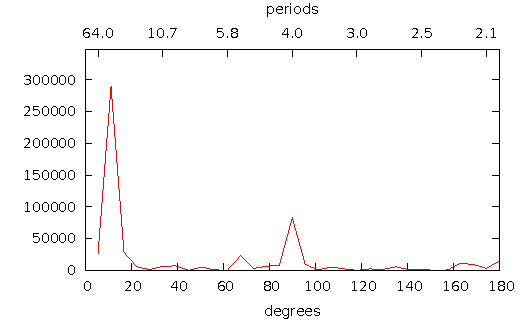
\includegraphics[scale=0.85]{figures/QNCpergm}} \\
  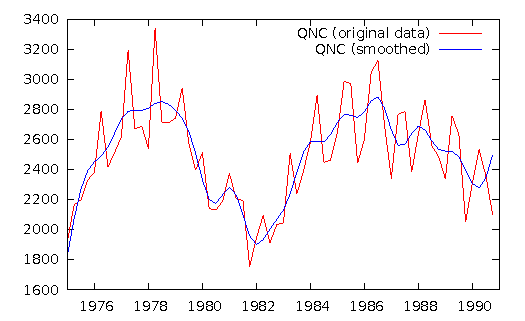
\includegraphics[scale=0.85]{figures/QNCfilt} &
\vbox{\hbox{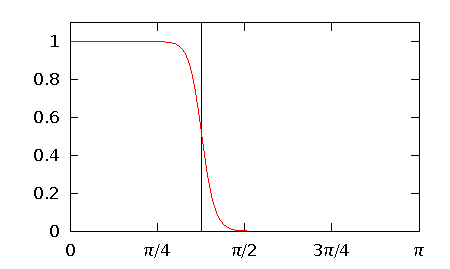
\includegraphics[scale=0.8]{figures/filtergain}}\vskip .3in}
\end{tabular}
\caption{The Butterworth filter applied}
\label{fig:QNCfilt}
\end{figure}

A seasonal pattern is clearly visible in the periodogram, centered at
an angle of 90$^{\circ}$ or 4 periods. If we set $\omega^{\star} =
68^{\circ}$ (or thereabouts) we should be able to excise the
seasonality quite cleanly using $n=8$.  The result is shown in the
lower panel of the Figure, along with the frequency response or gain
plot for the chosen filter. Note the smooth and reasonably steep
drop-off in gain centered on the nominal cutoff of $68^{\circ} \approx
3\pi/8$.

The apparatus that supports this sort of analysis in the \app{gretl}
GUI can be found under the \textsf{Variable} menu in the main window:
the items \textsf{Periodogram} and \textsf{Filter}. In the periodogram
dialog box you have the option of expressing the frequency axis in
degrees, which is helpful when selecting a Butterworth filter; and in
the Butterworth filter dialog you have the option of plotting the
frequency response as well as the smoothed series and/or the residual
or cycle.

     
\section{Panel data specifics}
\label{panel-genr}

\subsection{Dummy variables}
\label{dummies}

In a panel study you may wish to construct dummy variables of one or
both of the following sorts: (a) dummies as unique identifiers for the
units or groups, and (b) dummies as unique identifiers for the time
periods.  The former may be used to allow the intercept of the
regression to differ across the units, the latter to allow the
intercept to differ across periods.

Two special functions are available to create such dummies.  These are
found under the ``Add'' menu in the GUI, or under the \cmd{genr}
command in script mode or \app{gretlcli}.

\begin{enumerate}
\item ``unit dummies'' (script command \cmd{genr unitdum}).  This
  command creates a set of dummy variables identifying the
  cross-sectional units.  The variable \verb+du_1+ will have value 1
  in each row corresponding to a unit 1 observation, 0 otherwise;
  \verb+du_2+ will have value 1 in each row corresponding to a unit 2
  observation, 0 otherwise; and so on.
\item ``time dummies'' (script command \cmd{genr timedum}).  This
  command creates a set of dummy variables identifying the periods.
  The variable \verb+dt_1+ will have value 1 in each row
  corresponding to a period 1 observation, 0 otherwise; \verb+dt_2+
  will have value 1 in each row corresponding to a period 2
  observation, 0 otherwise; and so on.
\end{enumerate}

If a panel data set has the \verb+YEAR+ of the observation entered as
one of the variables you can create a periodic dummy to pick out a
particular year, e.g.\ \cmd{genr dum = (YEAR=1960)}.  You can also
create periodic dummy variables using the modulus operator,
\verb+%+.  For instance, to create a dummy with
value 1 for the first observation and every thirtieth observation
thereafter, 0 otherwise, do
%
\begin{code}
genr index 
genr dum = ((index-1) % 30) = 0
\end{code}

\subsection{Lags, differences, trends}
\label{panel-lagged}

If the time periods are evenly spaced you may want to use lagged
values of variables in a panel regression (but see also
chapter~\ref{chap-dpanel}); you may also wish to construct first
differences of variables of interest.

Once a dataset is identified as a panel, \app{gretl} will handle the
generation of such variables correctly.  For example the command
\verb+genr x1_1 = x1(-1)+ will create a variable that contains the
first lag of \verb+x1+ where available, and the missing value code
where the lag is not available (e.g.\ at the start of the time series
for each group).  When you run a regression using such variables, the
program will automatically skip the missing observations.

When a panel data set has a fairly substantial time dimension, you may
wish to include a trend in the analysis.  The command \cmd{genr time} 
creates a variable named \varname{time} which runs from 1 to $T$ for
each unit, where $T$ is the length of the time-series dimension of the
panel.  If you want to create an index that runs consecutively from 1
to $m\times T$, where $m$ is the number of units in the panel, use
\cmd{genr index}.

\subsection{Basic statistics by unit}
\label{panel-stats}

\app{Gretl} contains functions which can be used to generate basic
descriptive statistics for a given variable, on a per-unit basis;
these are \texttt{pnobs()} (number of valid cases), \texttt{pmin()}
and \texttt{pmax()} (minimum and maximum) and \texttt{pmean()} and
\texttt{psd()} (mean and standard deviation).

As a brief illustration, suppose we have a panel data set comprising 8
time-series observations on each of $N$ units or groups.  Then the
command
%
\begin{code}
genr pmx = pmean(x)
\end{code}
%
creates a series of this form: the first 8 values (corresponding to
unit 1) contain the mean of \varname{x} for unit 1, the next 8 values
contain the mean for unit 2, and so on.  The \texttt{psd()} function
works in a similar manner.  The sample standard deviation for group
$i$ is computed as
\[
s_i = \sqrt{\frac{\sum(x-\bar{x}_i)^2}{T_i-1}}
\]
where $T_i$ denotes the number of valid observations on \varname{x}
for the given unit, $\bar{x}_i$ denotes the group mean, and the
summation is across valid observations for the group.  If $T_i < 2$,
however, the standard deviation is recorded as 0.

One particular use of \texttt{psd()} may be worth noting.  If you want
to form a sub-sample of a panel that contains only those units for
which the variable \varname{x} is time-varying, you can either use 
%
\begin{code}
smpl (pmin(x) < pmax(x)) --restrict
\end{code}
or
%
\begin{code}
smpl (psd(x) > 0) --restrict
\end{code}

\subsection{Special functions for data manipulation}
\label{panel-manip}

Besides the functions discussed above, there are some facilities in
\texttt{genr} designed specifically for manipulating panel data --- in
particular, for the case where the data have been read into the
program from a third-party source and they are not in the correct
form for panel analysis.  These facilities are explained in
Chapter~\ref{datafiles}.


\section{Resampling and bootstrapping}
\label{sec:genr-resample}

Another specialized function is the resampling, with replacement, of a
series.  Given an original data series \varname{x}, the command
%
\begin{code}
genr xr = resample(x)
\end{code}
%
creates a new series each of whose elements is drawn at random from
the elements of \varname{x}.  If the original series has 100
observations, each element of \varname{x} is selected with probability
$1/100$ at each drawing.  Thus the effect is to ``shuffle'' the
elements of \varname{x}, with the twist that each element of
\varname{x} may appear more than once, or not at all, in \varname{xr}.

The primary use of this function is in the construction of bootstrap
confidence intervals or p-values.  Here is a simple example.  Suppose
we estimate a simple regression of $y$ on $x$ via OLS and find that
the slope coefficient has a reported $t$-ratio of 2.5 with 40 degrees
of freedom.  The two-tailed p-value for the null hypothesis that the
slope parameter equals zero is then 0.0166, using the $t(40)$
distribution.  Depending on the context, however, we may doubt whether
the ratio of coefficient to standard error truly follows the $t(40)$
distribution.  In that case we could derive a bootstrap p-value as
shown in Example~\ref{resampling-loop}.  

Under the null hypothesis that the slope with respect to $x$ is zero,
$y$ is simply equal to its mean plus an error term.  We simulate $y$
by resampling the residuals from the initial OLS and re-estimate the
model.  We repeat this procedure a large number of times, and record
the number of cases where the absolute value of the $t$-ratio is
greater than 2.5: the proportion of such cases is our bootstrap
p-value.  For a good discussion of simulation-based tests and
bootstrapping, see Davidson and MacKinnon
(\citeyear{davidson-mackinnon04}, chapter 4).

\begin{script}[htbp]
  \caption{Calculation of bootstrap p-value}
  \label{resampling-loop}
\begin{scode}
ols y 0 x
# save the residuals
genr ui = $uhat
scalar ybar = mean(y)
# number of replications for bootstrap
scalar replics = 10000
scalar tcount = 0
series ysim = 0
loop replics --quiet
  # generate simulated y by resampling
  ysim = ybar + resample(ui)
  ols ysim 0 x
  scalar tsim = abs($coeff(x) / $stderr(x))
  tcount += (tsim > 2.5)
endloop      
printf "proportion of cases with |t| > 2.5 = %g\n", tcount / replics
\end{scode}
%$
\end{script}

\section{Cumulative densities and p-values}
\label{sec:genr-cdf}

The two functions \cmd{cdf} and \cmd{pvalue} provide complementary
means of examining values from several probability distributions: the
standard normal, Student's $t$, $\chi^2$, $F$, gamma, and binomial.
The syntax of these functions is set out in the \GCR; here we expand
on some subtleties.

The cumulative density function or CDF for a random variable
is the integral of the variable's density from its lower limit
(typically either $-\infty$ or 0) to any specified value $x$.  The
p-value (at least the one-tailed, right-hand p-value as returned by
the \cmd{pvalue} function) is the complementary probability, the
integral from $x$ to the upper limit of the distribution, typically
$+\infty$.  

In principle, therefore, there is no need for two distinct functions:
given a CDF value $p_0$ you could easily find the corresponding
p-value as $1-p_0$ (or vice versa).  In practice, with
finite-precision computer arithmetic, the two functions are not
redundant.  This requires a little explanation.  In \app{gretl}, as in
most statistical programs, floating point numbers are represented as
``doubles'' --- double-precision values that typically have a storage
size of eight bytes or 64 bits.  Since there are only so many bits
available, only so many floating-point numbers can be represented:
\textit{doubles do not model the real line}.  Typically doubles can
represent numbers over the range (roughly) $\pm 1.7977 \times
10^{308}$, but only to about 15 digits of precision.

Suppose you're interested in the left tail of the $\chi^2$ distribution
with 50 degrees of freedom: you'd like to know the CDF value for $x =
0.9$.  Take a look at the following interactive session: 
\begin{code}
? genr p1 = cdf(X, 50, 0.9)
Generated scalar p1 (ID 2) = 8.94977e-35
? genr p2 = pvalue(X, 50, 0.9)
Generated scalar p2 (ID 3) = 1
? genr test = 1 - p2
Generated scalar test (ID 4) = 0
\end{code}

The \cmd{cdf} function has produced an accurate value, but the
\cmd{pvalue} function gives an answer of 1, from which it is not
possible to retrieve the answer to the CDF question.  This may seem
surprising at first, but consider: if the value of \texttt{p1} above
is correct, then the correct value for \texttt{p2} is $1 - 8.94977
\times 10^{-35}$.  But there's no way that value can be represented as
a double: that would require over 30 digits of precision.

Of course this is an extreme example.  If the $x$ in question is not
too far off into one or other tail of the distribution, the \cmd{cdf}
and \cmd{pvalue} functions will in fact produce complementary
answers, as shown below:
\begin{code}
? genr p1 = cdf(X, 50, 30)
Generated scalar p1 (ID 2) = 0.0111648
? genr p2 = pvalue(X, 50, 30)
Generated scalar p2 (ID 3) = 0.988835
? genr test = 1 - p2
Generated scalar test (ID 4) = 0.0111648
\end{code}
But the moral is that if you want to examine extreme values
you should be careful in selecting the function you need, in the
knowledge that values very close to zero can be represented as doubles
while values very close to 1 cannot.


\section{Handling missing values}
\label{sec:genr-missing}

Four special functions are available for the handling of missing
values.  The boolean function \verb+missing()+ takes the name of a
variable as its single argument; it returns a series with value 1 for
each observation at which the given variable has a missing value, and
value 0 otherwise (that is, if the given variable has a valid value at
that observation).  The function \verb+ok()+ is complementary to
\verb+missing+; it is just a shorthand for \verb+!missing+ (where
\verb+!+ is the boolean NOT operator).  For example, one can count the
missing values for variable \verb+x+ using

\begin{code}
genr nmiss_x = sum(missing(x))
\end{code}

The function \verb+zeromiss()+, which again takes a single series as
its argument, returns a series where all zero values are set to the
missing code.  This should be used with caution --- one does not want
to confuse missing values and zeros --- but it can be useful in some
contexts.  For example, one can determine the first valid observation
for a variable \verb+x+ using

\begin{code}
genr time
genr x0 = min(zeromiss(time * ok(x)))
\end{code}

The function \verb+misszero()+ does the opposite of \verb+zeromiss+,
that is, it converts all missing values to zero.  

It may be worth commenting on the propagation of missing values within
\verb+genr+ formulae.  The general rule is that in arithmetical
operations involving two variables, if either of the variables has a
missing value at observation $t$ then the resulting series will also
have a missing value at $t$.  The one exception to this rule is
multiplication by zero: zero times a missing value produces zero
(since this is mathematically valid regardless of the unknown value).
    

\section{Retrieving internal variables}
\label{sec:genr-internal}

The \verb+genr+ command provides a means of retrieving various values
calculated by the program in the course of estimating models or
testing hypotheses.  The variables that can be retrieved in this way
are listed in the \GCR; here we say a bit more about the special
variables \dollar{test} and \dollar{pvalue}.

These variables hold, respectively, the value of the last test
statistic calculated using an explicit testing command and the p-value
for that test statistic.  If no such test has been performed at the
time when these variables are referenced, they will produce the
missing value code.  The ``explicit testing commands'' that work in
this way are as follows: \cmd{add} (joint test for the significance of
variables added to a model); \cmd{adf} (Augmented Dickey--Fuller test,
see below); \cmd{arch} (test for ARCH); \cmd{chow} (Chow test for a
structural break); \cmd{coeffsum} (test for the sum of specified
coefficients); \cmd{cusum} (the Harvey--Collier $t$-statistic);
\cmd{kpss} (KPSS stationarity test, no p-value available);
\cmd{lmtest} (see below); \cmd{meantest} (test for difference of
means); \cmd{omit} (joint test for the significance of variables
omitted from a model); \cmd{reset} (Ramsey's RESET); \cmd{restrict}
(general linear restriction); \cmd{runs} (runs test for randomness);
\cmd{testuhat} (test for normality of residual); and \cmd{vartest}
(test for difference of variances). In most cases both a \dollar{test}
and a \dollar{pvalue} are stored; the exception is the KPSS test, for
which a p-value is not currently available.
    
An important point to notice about this mechanism is that the internal
variables \dollar{test} and \dollar{pvalue} are over-written each time
one of the tests listed above is performed.  If you want to reference
these values, you must do so at the correct point in the sequence of
\app{gretl} commands.  

A related point is that some of the test commands generate, by
default, more than one test statistic and p-value; in these cases only
the last values are stored. To get proper control over the retrieval
of values via \dollar{test} and \dollar{pvalue} you should formulate the
test command in such a way that the result is unambiguous.  This
comment applies in particular to the \verb+adf+ and \verb+lmtest+
commands.

\begin{itemize}
\item By default, the \cmd{adf} command generates three variants of
  the Dickey--Fuller test: one based on a regression including a
  constant, one using a constant and linear trend, and one using a
  constant and a quadratic trend.  When you wish to reference
  \dollar{test} or \dollar{pvalue} in connection with this command, you
  can control the variant that is recorded by using one of the flags
  \option{nc}, \option{c}, \option{ct} or \option{ctt} with
  \verb+adf+.
\item By default, the \cmd{lmtest} command (which must follow an OLS
  regression) performs several diagnostic tests on the regression in
  question.  To control what is recorded in \dollar{test} and
  \dollar{pvalue} you should limit the test using one of the flags
  \option{logs}, \option{autocorr}, \option{squares} or
  \option{white}.
\end{itemize}

As an aid in working with values retrieved using \dollar{test} and
\dollar{pvalue}, the nature of the test to which these values relate is
written into the descriptive label for the generated variable.  You
can read the label for the variable using the \cmd{label} command
(with just one argument, the name of the variable), to check that you
have retrieved the right value.  The following interactive session
illustrates this point.

\begin{code}
? adf 4 x1 --c
Augmented Dickey-Fuller tests, order 4, for x1
sample size 59
unit-root null hypothesis: a = 1
  test with constant
  model: (1 - L)y = b0 + (a-1)*y(-1) + ... + e
  estimated value of (a - 1): -0.216889
  test statistic: t = -1.83491
  asymptotic p-value 0.3638
P-values based on MacKinnon (JAE, 1996)
? genr pv = $pvalue
Generated scalar pv (ID 13) = 0.363844
? label pv    
  pv=Dickey-Fuller pvalue (scalar)
\end{code}
%$

\section{Numerical procedures}
\label{sec:genr-numerical}

Two special functions are available to aid in the construction of
special-purpose estimators, namely \texttt{BFGSmax} (the BFGS
maximizer, discussed in Chapter~\ref{chap:mle}) and \texttt{fdjac},
which produces a forward-difference approximation to the Jacobian.

\subsection{The BFGS maximizer}
\label{sec:BFGSmax}

The \texttt{BFGSmax} function has two required arguments: a vector
holding the initial values of a set of parameters, and a call to a
function that calculates the (scalar) criterion to be maximized, given
the current parameter values and any other relevant data.  If the
object is in fact minimization, this function should return the
negative of the criterion.  On successful completion, \texttt{BFGSmax}
returns the maximized value of the criterion and the matrix given via
the first argument holds the parameter values which produce the
maximum.  Here is an example:
%
\begin{code}
matrix X = { dataset }
matrix theta = { 1, 100 }'
scalar J = BFGSmax(theta, ObjFunc(&theta, &X))
\end{code}
%
It is assumed here that \texttt{ObjFunc} is a user-defined function
(see Chapter~\ref{chap:functions}) with the following general set-up:
%
\begin{code}
function scalar ObjFunc (matrix *theta, matrix *X)
  scalar val = ...  # do some computation
  return val
end function
\end{code}

\begin{script}[htbp]
  \caption{Finding the minimum of the Rosenbrock function}
  \label{rosenbrock}
\begin{scode}
function scalar Rosenbrock(matrix *param)
  scalar x = param[1]
  scalar y = param[2]
  return -(1-x)^2 - 100 * (y - x^2)^2
end function

matrix theta = { 0 , 0 }

set max_verbose 1
M = BFGSmax(theta, Rosenbrock(&theta))

print theta
\end{scode}
\end{script}

The operation of the BFGS maximizer can be adjusted using the
\texttt{set} variables \verb+bfgs_maxiter+ and \verb+bfgs_toler+ (see
Chapter~\ref{chap:mle}).  In addition you can provoke verbose output
from the maximizer by assigning a positive value to
\verb|max_verbose|, again via the \texttt{set} command.

The Rosenbrock function is often used as a test problem for
optimization algorithms. It is also known as ``Rosenbrock's Valley''
or ``Rosenbrock's Banana Function'', on account of the fact that its
contour lines are banana-shaped. It is defined by:
%
\[
    f(x,y) = (1 - x)^2 + 100(y - x^2)^2
\]
%
The function has a global minimum at $(x,y) = (1,1)$ where $f(x,y) =
0$.  Example~\ref{rosenbrock} shows a \app{gretl} script that
discovers the minimum using \texttt{BFGSmax} (giving a verbose account
of progress).  

\subsection{Supplying analytical derivatives for BFGS}
\label{sec:BFGSgrad}

An optional third argument to the \texttt{BFGSmax} function enables
the user to supply analytical derivatives of the criterion
function with respect to the parameters (without which a numerical
approximation to the gradient is computed).  This argument is
similar to the second one in that it specifies a function call.
In this case the function that is called must have the following
signature.  

Its first argument should be a pre-defined matrix correctly
dimensioned to hold the gradient; that is, if the parameter vector
contains $k$ elements, the gradient matrix must also be a $k$-vector.
This matrix argument must be given in ``pointer'' form so that its
content can be modified by the function.  (Note that unlike the
parameter vector, where the choice of initial values can be important,
the initial values given to the gradient are immaterial and do not
affect the results.)

In addition the gradient function must have as one of its argument the
parameter vector.  This may be given in pointer form (which enhances
eficiency) but that is not required.  Additional arguments may be
specified if necessary.

Given the current parameter values, the function call must fill out
the gradient vector appropriately.  It is not required that the
gradient function returns any value directly; if it does, that value
is ignored.

Example~\ref{rosen-analytical} illustrates, showing how the Rosenbrock
script can be modified to use analytical derivatives.  (Note that
since this is a minimization problem the values written into
\texttt{g[1]} and \texttt{g[2]} in the function \verb|Rosen_grad| are
in fact the derivatives of the negative of the Rosenbrock function.)

\begin{script}[htbp]
  \caption{Rosenbrock function with analytical gradient}
  \label{rosen-analytical}
\begin{scode}
function scalar Rosenbrock (matrix *param)
  scalar x = param[1]
  scalar y = param[2]
  return -(1-x)^2 - 100 * (y - x^2)^2
end function

function void Rosen_grad (matrix *g, matrix *param)
  scalar x = param[1]
  scalar y = param[2]
  g[1] = 2*(1-x) + 2*x*(200*(y-x^2))
  g[2] = -200*(y - x^2)
end function

matrix theta = { 0, 0 }
matrix grad = { 0, 0 }

set max_verbose 1
M = BFGSmax(theta, Rosenbrock(&theta), Rosen_grad(&grad, &theta))

print theta
print grad
\end{scode}
\end{script}

\subsection{Computing a Jacobian}
\label{sec:fdjac}

\app{Gretl} offers the possibility of differentiating numerically a
user-defined function via the \texttt{fdjac} function. 

This function again takes two arguments: an $n \times 1$ matrix
holding initial parameter values and a function call that calculates
and returns an $m \times 1$ matrix, given the current parameter values
and any other relevant data.  On successful completion it returns an
$m \times n$ matrix holding the Jacobian.  For example,
%
\begin{code}
matrix Jac = fdjac(theta, SumOC(&theta, &X))
\end{code}
where we assume that \texttt{SumOC} is a user-defined function with
the following structure:
%
\begin{code}
function matrix SumOC (matrix *theta, matrix *X)
  matrix V = ...  # do some computation
  return V
end function
\end{code}

This may come in handy in several cases: for example, if you use
\texttt{BFGSmax} to estimate a model, you may wish to calculate a
numerical approximation to the relevant Jacobian to construct a
covariance matrix for your estimates.

Another example is the delta method: if you have a consistent
estimator of a vector of parameters $\hat{\theta}$, and a consistent
estimate of its covariance matrix $\Sigma$, you may need to compute
estimates for a nonlinear continuous transformation $\psi =
g(\theta)$. In this case, a standard result in asymptotic theory is
that
\[
\left\{
    \begin{array}{c}
      \hat{\theta} \convp \theta \\ 
      \sqrt{T} \left( \hat{\theta} - \theta \right) \convd N(0, \Sigma)
    \end{array}
\right\}
    \Longrightarrow
\left\{
    \begin{array}{c}
      \hat{\psi} = g(\hat{\theta}) \convp \psi = g(\theta) \\ 
      \sqrt{T} \left( \hat{\psi} - \psi \right) \convd N(0, J
      \Sigma J')
    \end{array}
\right\}
\]
where $T$ is the sample size and $J$ is the Jacobian
$\left.\pder{g(x)}{x}\right|_{x = \theta}$.

\begin{script}[htbp]
  \caption{Delta Method}
  \label{delta-method}
\begin{scode}
function matrix MPC(matrix *param, matrix *Y)
  beta = param[2]
  gamma = param[3]
  y = Y[1]
  return beta*gamma*y^(gamma-1)
end function

# William Greene, Econometric Analysis, 5e, Chapter 9
set echo off
set messages off
open greene5_1.gdt

# Use OLS to initialize the parameters
ols realcons 0 realdpi --quiet
genr a = $coeff(0)
genr b = $coeff(realdpi)
genr g = 1.0

# Run NLS with analytical derivatives
nls realcons = a + b * (realdpi^g)
  deriv a = 1
  deriv b = realdpi^g
  deriv g = b * realdpi^g * log(realdpi)
end nls

matrix Y = realdpi[2000:4]
matrix theta = $coeff
matrix V = $vcv

mpc = MPC(&theta, &Y)
matrix Jac = fdjac(theta, MPC(&theta, &Y))
Sigma = qform(Jac, V)

printf "\nmpc = %g, std.err = %g\n", mpc, sqrt(Sigma)
scalar teststat = (mpc-1)/sqrt(Sigma)
printf "\nTest for MPC = 1: %g (p-value = %g)\n", \
	teststat, pvalue(n,abs(teststat))
\end{scode}
\end{script}

Script \ref{delta-method} exemplifies such a case: the example is
taken from \cite{greene03}, section 9.3.1. The slight differences
between the results reported in the original source and what
\app{gretl} returns are due to the fact that the Jacobian is computed
numerically, rather than analytically as in the book.

\section{The discrete Fourier transform}
\label{sec:genr-fft}

The discrete Fourier transform can be best thought of as a linear,
invertible transform of a complex vector. Hence, if $\mathbf{x}$ is an
$n$-dimensional vector whose $k$-th element is $x_k = a_k + i b_k$,
then the output of the discrete Fourier transform is a vector
$\mathbf{f} = \mathcal{F}(\mathbf{x})$ whose $k$-th element is
\[
  f_k = \sum_{j=0}^{n-1} e^{-i \omega(j,k) } x_j 
\]
where $\omega(j,k) = 2 \pi i \frac{j k}{n}$. Since the transformation
is invertible, the vector $\mathbf{x}$ can be recovered from
$\mathbf{f}$ via the so-called inverse transform
\[
  x_k = \frac{1}{n} \sum_{j=0}^{n-1} e^{i \omega(j,k) } f_j .
\]

The Fourier transform is used in many diverse situations
on account of this key property: the convolution of two vectors can be
performed efficiently by multiplying the elements of their Fourier
transforms and inverting the result.  If
\[
  z_k = \sum_{j=1}^n x_j y_{k-j} ,
\]
then
\[
  \mathcal{F}(\mathbf{z}) = \mathcal{F}(\mathbf{x}) \odot
  \mathcal{F}(\mathbf{y}) .
\]
That is, $\mathcal{F}(\mathbf{z})_k = \mathcal{F}(\mathbf{x})_k
\mathcal{F}(\mathbf{y})_k$.

For computing the Fourier transform, \app{gretl} uses the external
library \texttt{fftw3}: see \cite{frigo05}. This guarantees
extreme speed and accuracy. In fact, the CPU time needed to perform
the transform is $O(n \log n)$ for any $n$. This is why the array of
numerical techniques employed in \texttt{fftw3} is commonly known as
the \emph{Fast} Fourier Transform.

\app{Gretl} provides two matrix functions\footnote{See chapter
  \ref{chap:matrices}.} for performing the Fourier transform and its
inverse: \texttt{fft} and \texttt{ffti}. In fact, \app{gretl}'s
implementation of the Fourier transform is somewhat more specialized:
the input to the \texttt{fft} function is understood to be real.
Conversely, \texttt{ffti} takes a complex argument and delivers a real
result. For example:
\begin{code}
x1 = { 1 ; 2 ; 3 }
# perform the transform
f = fft(a)
# perform the inverse transform
x2 = ffti(f)
\end{code}
yields
\[
  x_1 = \left[ \begin{array}{c} 1 \\ 2 \\ 3 \end{array} \right] 
  \qquad
  f = \left[ \begin{array}{rr} 
      6 & 0 \\ -1.5 & 0.866 \\ -1.5 & -0.866 
   \end{array} \right] 
  \qquad
  x_2 = \left[ \begin{array}{c} 1 \\ 2 \\ 3 \end{array} \right] 
\]
where the first column of \emph{f} holds the real part and the second
holds the complex part. In general, if the input to \texttt{fft} has
$n$ columns, the output has $2n$ columns, where the real parts are
stored in the odd columns and the complex parts in the even
ones. Should it be necessary to compute the Fourier transform on
several vectors with the same number of elements, it is numerically more
efficient to group them into a matrix rather than invoking
\texttt{fft} for each vector separately.

As an example, consider the multiplication of two polynomals:
\begin{eqnarray*}
  a(x) & = & 1 + 0.5 x \\
  b(x) & = & 1 + 0.3 x - 0.8 x^2 \\
  c(x) = a(x) \cdot b(x) & = & 1 + 0.8 x - 0.65 x^2 - 0.4 x^3
\end{eqnarray*}
The coefficients of the polynomial $c(x)$ are the convolution of the
coefficents of $a(x)$ and $b(x)$; the following \app{gretl} code fragment
illustrates how to compute the coefficients of $c(x)$:
\begin{code}
# define the two polynomials
a = { 1, 0.5, 0, 0 }'
b = { 1, 0.3, -0.8, 0 }'
# perform the transforms
fa = fft(a)
fb = fft(b)
# complex-multiply the two transforms 
fc = cmult(fa, fb)
# compute the coefficients of c via the inverse transform
c = ffti(fc)
\end{code}

Maximum efficiency would have been achieved by grouping \texttt{a} and
\texttt{b} into a matrix.  The computational advantage is so little in
this case that the exercise is a bit silly, but the following
alternative may be preferable for a large number of
rows/columns:
\begin{code}
# define the two polynomials
a = { 1 ; 0.5; 0 ; 0 }
b = { 1 ; 0.3 ; -0.8 ; 0 }
# perform the transforms jointly
f = fft(a ~ b)
# complex-multiply the two transforms 
fc = cmult(f[,1:2], f[,3:4])
# compute the coefficients of c via the inverse transform
c = ffti(fc)
\end{code}

Traditionally, the Fourier tranform in econometrics has been mostly
used in time-series analysis, the periodogram being the best known
example. Example script \ref{scr:pergm-fft} shows how to compute the
periodogram of a time series via the \texttt{fft} function.

\begin{script}[htbp]
  \caption{Periodogram via the Fourier transform}
  \label{scr:pergm-fft}
\begin{scode}
nulldata 50
# generate an AR(1) process
series e = normal()
series x = 0
x = 0.9*x(-1) + e
# compute the periodogram
scale = 2*pi*$nobs
X = { x }
F = fft(X)
S = sumr(F.^2)
S = S[2:($nobs/2)+1]/scale
omega = seq(1,($nobs/2))' .* (2*pi/$nobs)
omega = omega ~ S
# compare the built-in command
pergm x  
print omega
\end{scode}
\end{script}

%%% Local Variables: 
%%% mode: latex
%%% TeX-master: "gretl-guide"
%%% End: 

